%%%%%%%%%%%%%%%%%%%%%%%%%%%%%%%%%%%%%%%%%
% Simple Sectioned Essay Template
% LaTeX Template
%
% This template has been downloaded from:
% http://www.latextemplates.com
%
% Note:
% The \lipsum[#] commands throughout this template generate dummy text
% to fill the template out. These commands should all be removed when 
% writing essay content.
%
%%%%%%%%%%%%%%%%%%%%%%%%%%%%%%%%%%%%%%%%%

%----------------------------------------------------------------------------------------
%	PACKAGES AND OTHER DOCUMENT CONFIGURATIONS
%----------------------------------------------------------------------------------------

\documentclass[12pt]{article} % Default font size is 12pt, it can be changed here
\usepackage[english]{babel}
\usepackage[utf8]{inputenc}
\usepackage{listings}
\usepackage{color}
\usepackage{caption}
%\usepackage[dvips]{graphicx}
\usepackage{geometry} % Required to change the page size to A4
%\geometry{a4paper} % Set the page size to be A4 as opposed to the default US Letter
\usepackage{framed}
\usepackage{url}
\usepackage{graphicx} % Required for including pictures
\usepackage{natbib}
\usepackage{float} % Allows putting an [H] in \begin{figure} to specify the exact location of the figure
%\usepackage{wrapfig} % Allows in-line images such as the example fish picture
\usepackage{hyperref}

\usepackage{fancyhdr}
\pagestyle{fancy}
\fancyhf{}
\fancyhead[RO]{{Initial Volume Estimation Tutorial}} 
\fancyhead[LO]{Scipion}
%\fancyhead[RO]{{\leftmark}} 
\fancyfoot[LE,RO]{{ \thepage }}

%\usepackage{lipsum} % Used for inserting dummy 'Lorem ipsum' text into the template
\definecolor{grey}{rgb}{0.9,0.9,0.9}

\linespread{1.2} % Line spacing

%\setlength\parindent{0pt} % Uncomment to remove all indentation from paragraphs

\newcounter{ejercicioNo}
\begin{document}

%----------------------------------------------------------------------------------------
%	TITLE PAGE
%----------------------------------------------------------------------------------------

\begin{titlepage}

\newcommand{\HRule}{\rule{\linewidth}{0.5mm}} % Defines a new command for the horizontal lines, change thickness here

\center % Center everything on the page

\textsc{\LARGE National Center for Biothecnology}\\[1.5cm] % Name of your university/college
%\textsc{\Large Proyecto de Sistemas Informaticos}\\[0.5cm] % Major heading such as course name
%\textsc{\large Departamento de Informática}\\[0.5cm] % Minor heading such as course title
\textsc{\Large Biocomputing Unit}\\[0.5cm] % Minor heading such as course title

\HRule \\[0.4cm]
{ \huge \bfseries Initial Volume Estimation Tutorial}\\[0.4cm] % Title of your document
\HRule \\[1.5cm]

%\begin{minipage}{0.4\textwidth}
%\begin{flushleft}
% \large
%\emph{Author:}\\
%Laura  \textsc{del Caño} % Your name
%\end{flushleft}
%\end{minipage}

%\begin{minipage}{0.4\textwidth}
%\begin{flushright} \large
%\emph{Supervisor:} \\
%Jose Miguel \textsc{de la Rosa} % Supervisor's Name
%\end{flushright}
%\end{minipage}\\[4cm]

%{\large \today}\\[3cm] % Date, change the \today to a set date if you want to be precise

%\includegraphics{Logo}\\[1cm] % Include a department/university logo - this will require the graphicx package

\vfill % Fill the rest of the page with whitespace
%\begin{minipage}{0.4\textwidth}
\begin{flushright}
 \large
%\emph{Author:}\\
  \textsc{Scipion Team} % Your name
\end{flushright}
%\end{minipage}

\end{titlepage}


%----------------------------------------------------------------------------------------
%	OBJETIVOS
%----------------------------------------------------------------------------------------



\subsection*{Intended audience}

This tutorial provides an introduction to initial volume estimation using Scipion. 
Very limited knowledge about 3D-EM image processing and Scipion is required, and basic computer skills.

\subsection*{We'd like to hear from you}

We have tested and verified the different steps described in this demo
to the best of our knowledge, but since our programs are in continuous
development you may find inaccuracies and errors in this text. Please,
let us know about any error you find, as well as your suggestions for
future editions by writing to
\href{mailto:scipion@cnb.csic.es}{scipion@cnb.csic.es}.

\newpage
%----------------------------------------------------------------------------------------
%	TABLE OF CONTENTS
%----------------------------------------------------------------------------------------

\tableofcontents % Include a table of contents

\newpage % Begins the essay on a new page instead of on the same page as the table of contents 


\section{General Introduction}

\subsection{Download and Install}

The first step before start working on your projects is to download and
install Scipion and all the related programs. At \href{http://scipionwiki.cnb.csic.es}{Scipion's website} 
there is all the information needed to download and install the package.

\subsection{Initial Volume estimation}

Single Particle Analysis (SPA) techniques can obtain three-dimensional (3D) maps of biological complexes 
at near atomic resolution by combining tens of thousands of projection images obtained on a 
Transmission Electron Microscopy (TEM). In general, the reconstruction process leading to the final 3D map 
requires the use of an approximate low resolution initial model to be refined in further steps. 
In this tutorial we present different methods to obtain this initial model using Scipion, 
which are Random Conical Tilt, 3D-RANSAC and Eman.

\section{Random Conical Tilt}

One of the most widespread Single Particle Analysis (SPA) techniques, inside the Transmission
Electron Microscopy (TEM) field, is the Random Conical Tilt (RCT) (see Radermacher et al. (1987)). 
In RCT, we assume that we have a randomly distributed particle in all its conformations and positions 
along a sample, so when we take a low power TEM image, we’re getting multiple views of the same particle. 
The specimen stage of the microscope is then tilted and a new low power TEM image is taken. 
The less power, the less exposure of the sample. This is a cryoEM constraint on biological objects. 
As a result, images with a low signal-to-noise ratio (SNR) are taken. With this 2 images, 
every processing program will need to relate each particle to its tilted version, 
in order to get different views of the specimen and estimate the tilt angle.

\begin{figure}
\centering
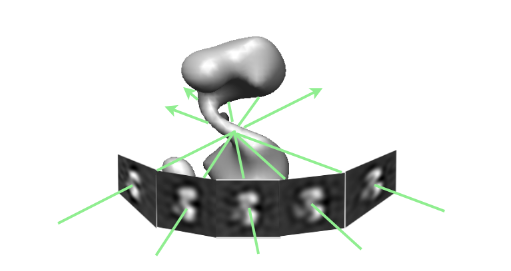
\includegraphics[width=0.75\textwidth]
{{images/01.RCTprojection}.png}
\caption{How the projections vary with the tilt.}
\label{RCTprojection}
\end{figure}

\subsection{Getting started}

The data you will work on may be downloaded using the following command:

\begin{verbatim}
scipion testdata --download rct
\end{verbatim}

The data will be download in \verb+scipion_folder/data/tests/sct+.

After download, you must launch the MAIN GUI by typing: \verb+scipion+
Then, create a new project by clicking \textbf{Create project} button, type a 
\textit{project name} and click OK. The GUI main project window will be launched.
On the left panel a view can be selected which contains different protocols grouped in categories. 
Clicking on a group will display a menu with protocols that can be selected to launch the
corresponding GUI.
To follow the tutorial you should select the \textbf{Random Conical Tilt} view on the upper left corner.

\subsection{Import tilted pairs micrographs}

The first step is to import the tilted pairs micrographs to your scipion project. To do this,
press on \textbf{Import Micrographs pairs} protocol. 
In \textit{Pattern untilted} and \textit{Pattern tilted}  you must indicate where your untilted 
and tilted micrograph files are stored (clicking on \textbf{browse} button). The complete patterns are:

\begin{verbatim}
$SCIPION_HOME/data/tests/rct/micrographs/F_rct_u_*.tif

$SCIPION_HOME/data/tests/rct/micrographs/F_rct_t_*.tif
\end{verbatim}


In this first version pairs assignment is done by micrograph order but in next versions a wizard 
will be provided.

Modify the parameters of the Import Micrographs protocol according to the ones
shown in figure~\ref{ImportMics}.

\begin{figure}
\centering
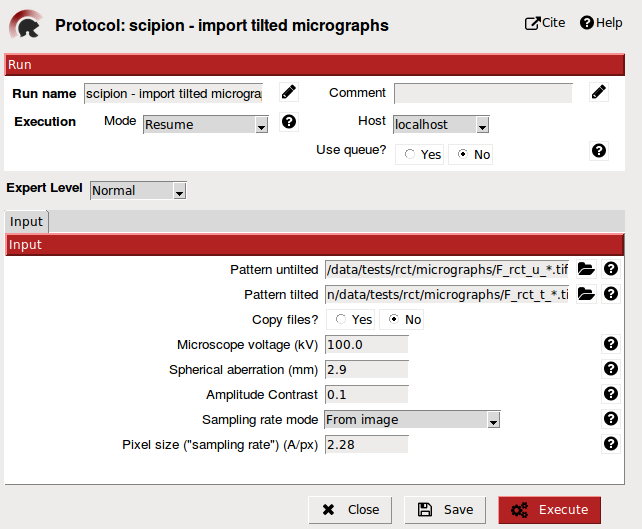
\includegraphics[width=0.75\textwidth]
{{images/02.ImportMics}.png}
\caption{Import Micrographs protocol GUI.}
\label{ImportMics}
\end{figure}

When you have completed the form, click on the \textbf{Execute} button. 

Once the protocol has finished you can press the \textbf{Analyze results} button and a new pop-up GUI will open
where you can see the imported micrographs pairs as shown in figure ~\ref{ImportResults}.

\begin{figure}
\centering
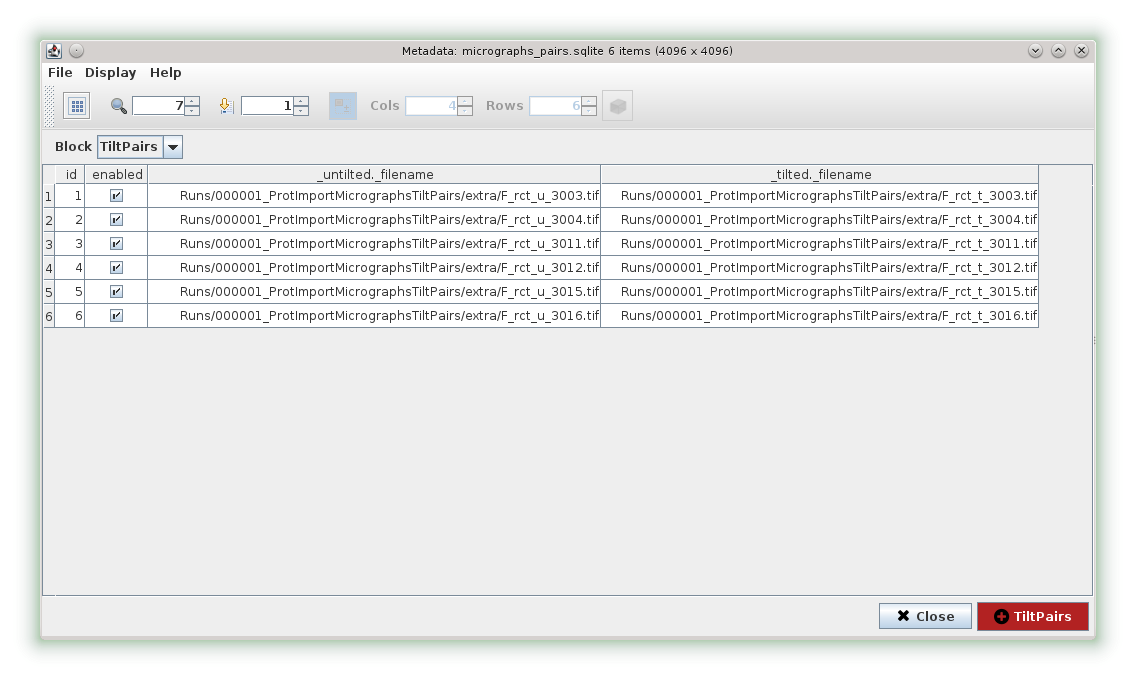
\includegraphics[width=0.75\textwidth]
{{images/03.ImportResults}.png}
\caption{Import Micrographs results.}
\label{ImportResults}
\end{figure}

\subsection{Particle Picking}
Once the micrographs have been imported you need to pick tilted and untilted particle pairs.
Press on \textbf{Picking micrographs pairs} protocol  and form shown in figure~\ref{PickingProtocol} 
will appear. Select the Micrographs Tilt Pair object produced by the import protocol as input and 
click on the \textbf{Execute} button. The Xmipp particle picking GUI will open.

If you find some particles difficult to see due to noise and contrast of the images, you can use the 
different filters offered by the Xmipp particle picking GUI on the \textbf{Filters} menu.
For instance you might select the \textbf{Brightness/Contrast} filter and press the \textbf{Auto} button that will 
set the brightness and contrast to the optimal values for the selected micrograh. Then change to other micrographs 
and do the same. The resulting interface will be much easier to start picking.

The picking procedure is:

1.  Find the first particle in both untilted and tilted. First pick the untilted and then its tilted
pair.

2.  Pick three more particles like the first one, having special care in correcting
the tilted one, so the tilt estimation can be properly set. During the first particles picking,
the manual error correction will help the algorithm to learn and propose a better tilt adjust-
ment. For detecting the error, it is better to zoom in the micrograph. Note that zooming in
or out in the untilted micrograph will replicate in the tilted one, but not in the other side.
To zoom in, press shift key and scroll up, to zoom out, press shift key and scroll down.

3.  Finally continue picking just the untilted (tilted will automatically be picked) but keeping
an eye on the tilted, in order to prevent from deviations due to accumulated error. The amount 
of particles to pick for a good reconstruction varies depending on the tilt angle,
the quality of the micrographs and many other factors, but a good approach to start could
be 2000 particles.

However if you don't feel like picking manually thousands of particles you can import the already picked 
particles by clicking on \textbf{File/Import coordinates} and specifying the following path.

\begin{verbatim}
$SCIPION_HOME/data/tests/rct/positions
\end{verbatim}

Take into account that the protocol status will not changed to \textbf{Finished} but remain as \textbf{Interactive}.
This allows you to execute it again if you wish to pick more particles.

\begin{figure}
\centering
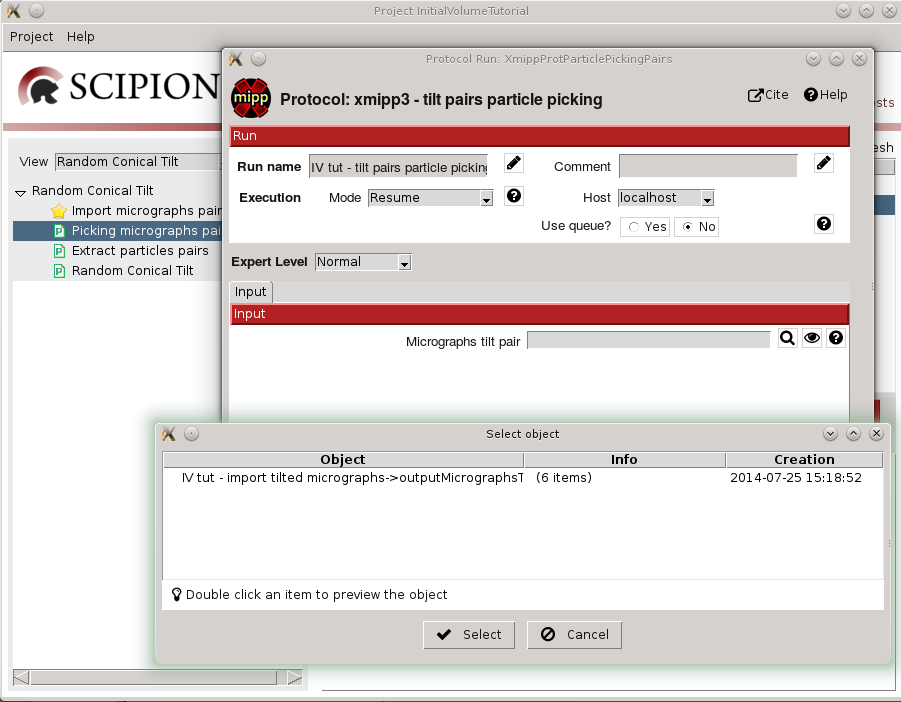
\includegraphics[width=0.75\textwidth]{{images/04.PickingProtocol}.png}
\caption{Picking pairs protocol}
\label{PickingProtocol}
\end{figure}

\begin{figure}
\centering
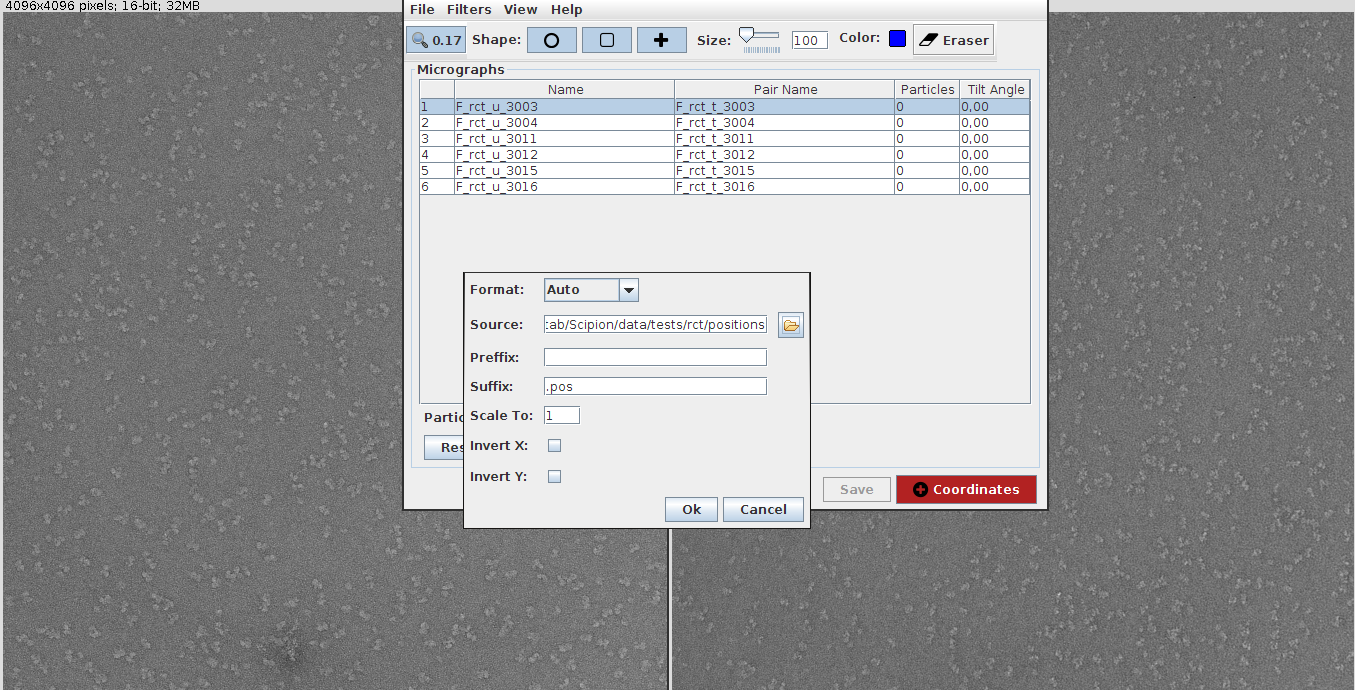
\includegraphics[width=0.75\textwidth]{{images/05.PickingGUI}.png}
\caption{Xmipp particle picking pairs GUI}
\label{PickingGUI}
\end{figure}

\subsection{Extract particles pairs}
Now that coordinates pairs are picked they have to be extracted as particle pairs.
To do so select the \textbf{Extract particles pairs} protocol and fill in the parameters as shown in figure~\ref{ExtractPairs}.
Although particles were picked with a size of 120 pixels the extract will downsample them on a factor of two to speed up next steps.

Once the protocol has finished you can review the particles by clicking on the \textbf{Analyze results} button as seen in figure~\ref{ExtractResults}.
If you don't like some of the particles you can disable them and create a subset with the good ones. Just click on the \textbf{TiltPairs} red button 
and give the subset a name.

\begin{figure}
\centering
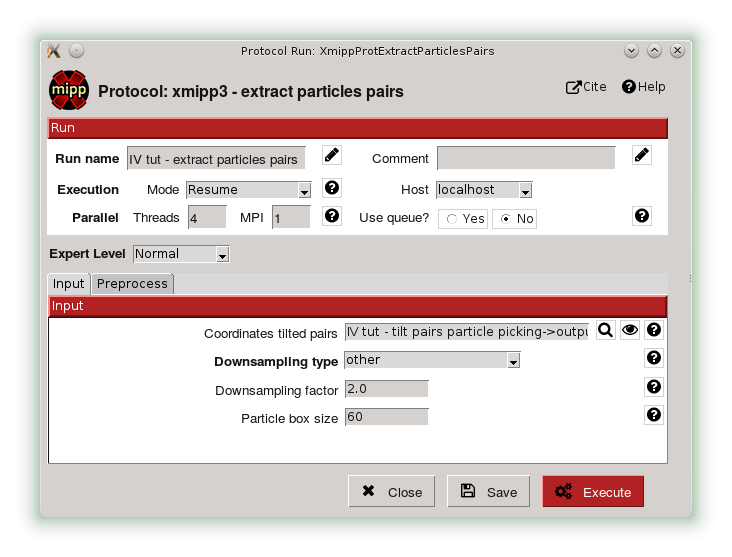
\includegraphics[width=0.75\textwidth]{{images/06.ExtractPairsProtocol}.png}
\caption{Extract particles pairs protocol}
\label{ExtractPairs}
\end{figure}

\begin{figure}
\centering
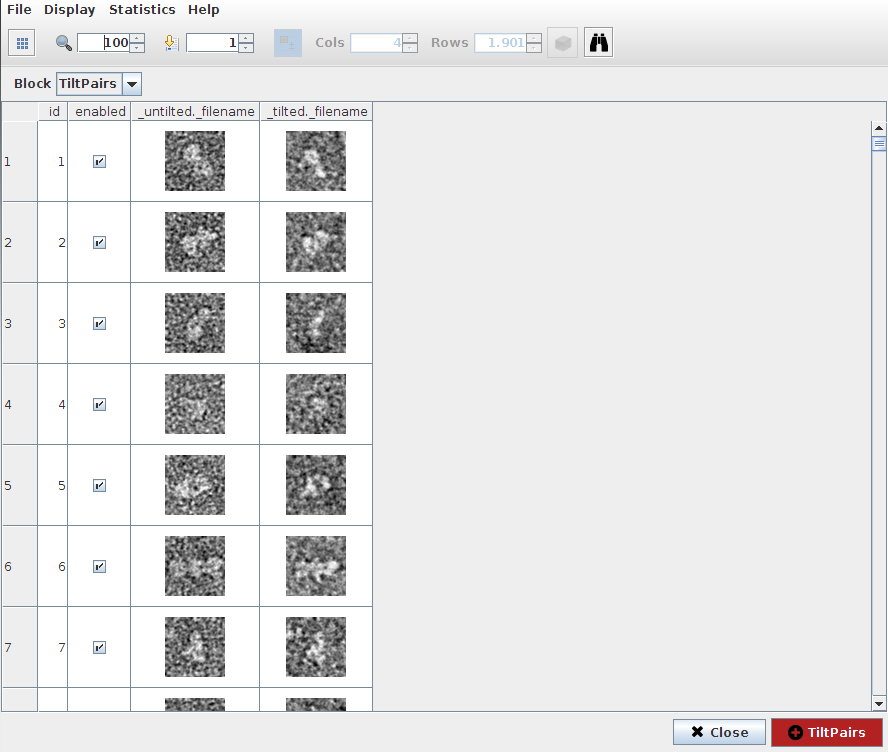
\includegraphics[width=0.75\textwidth]{{images/07.ExtractPairsResults}.png}
\caption{Extract particles pairs results}
\label{ExtractResults}
\end{figure}

\subsection{Classification with CL2D}
Once the particles are extracted, they have to be classified, in order to group those belonging to different state of the particle 
or even those which represent an error in the picking. For this tutorial you will perform a CL2D classification from Xmipp package.

Since this protocol is not exclusive of RCT you have to change view on the upper left menu and select \textbf{Protocols SPA}.
CL2D protocol is found under \textbf{2D - Classify}.

Select the set of untilted particles produced by the previous step or the ones on the subset if you chose to remove some of the particles.
Fill in the rest of the parameters as shown in figure~\ref{CL2D} and press \textbf{Execute}.

This protocol will take some time to finish (depending on your computer power and number of mpis choosen). Once it has finished you can 
visualize the classes obtained by clicking on \textbf{Analyze results} button.

This classes show mean images that represent your particles, but to be sure that they’re representing with fidelity your particle, 
at least some basic assessment steps are needed. 

Be sure you’re using the stable core classes. These are composed by those particles that have stayed through all iterations together. 

Each class should contain between 100 and 200 particles more or less. Less than 100 will result in reconstructions of low quality, 
so the estimation is not being properly done. Also, more than 200-250 particles would result in a wrong estimation because particles 
very different could be mixing in the same class. 

Some extra assessment can be done using the Principal Component Analysis (PCA) of the class images. 
PCA can be calculated by right clicking in the desired class and selecting “Open images”.
After that, images will show up (TODO: Ask AIREN how to perform this with showj if possible).

Apart from that, there is also a subjective assessment, and it comes from what the user is looking for. 
Each class shows you a mean image that can give you an idea of what you will find if you start a reconstruction with those images. 
The user must select those volumes that are more promising. In our case, we can discard, using this criteria, classes 3 and 7, 
that seem to show particles in a top view (or just one part of the particle).
Then, as done with particles extracted, you should create a subset of classes to be used as input for next step, 
as shown on figure~\ref{CL2Dresults}

\begin{figure}
\centering
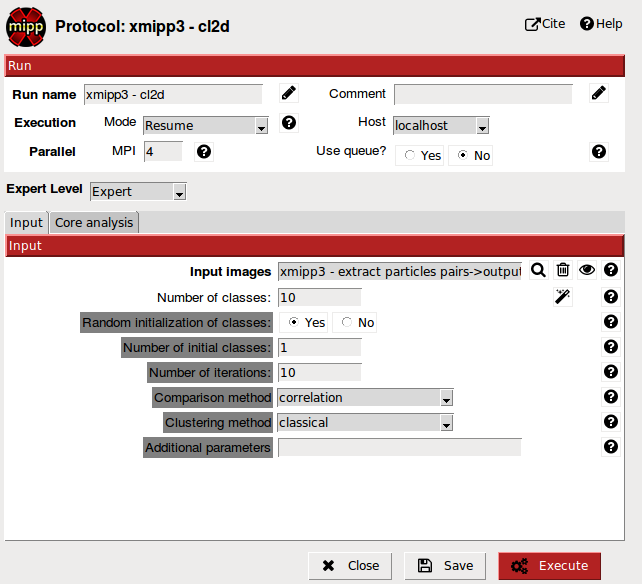
\includegraphics[width=0.75\textwidth]{{images/08.CL2Dprotocol}.png}
\caption{CL2D protocol}
\label{CL2D}
\end{figure}

\begin{figure}
\centering
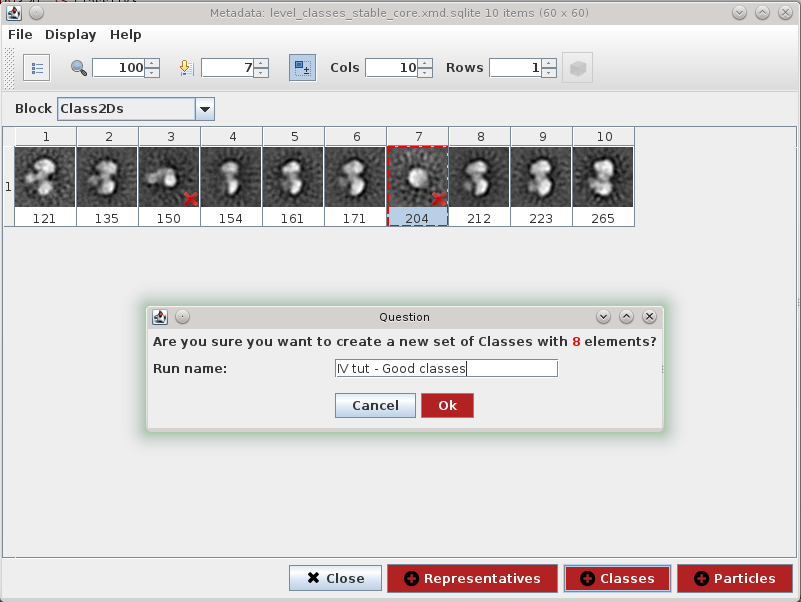
\includegraphics[width=0.75\textwidth]{{images/09.GoodClasses}.png}
\caption{CL2D results}
\label{CL2Dresults}
\end{figure}

\subsection{Initial volume generation with Random Conical Tilt}
Once you have the desired classes, only the RCT reconstruction step is left. 
Select \textbf{Random Conical Tilt} and fill in the form as shown in figure~\ref{RCTprotocol}.
You have to provide the particles tilt pair object produced by the extraction (or a subset) and the particles or classes 
you want to reconstruct. However if you choose particles they should contain alignment information.

The \textbf{Thin Object} option must be set to “Yes” if the particle is not more or less spherical. 
When the object is going to change its width significantly between the untilted and the tilted image, we can considered this a “thin object”. 

Reconstruction can also low-pass filter the volumes after the process is done, producing both filtered and not filtered volumes as output.
In order to visualize the volumes click on \textbf{Analyze results} after the protocol has finished, and a window as the one on figure~\ref{RCTresults} 
will show up.

\begin{figure}
\centering
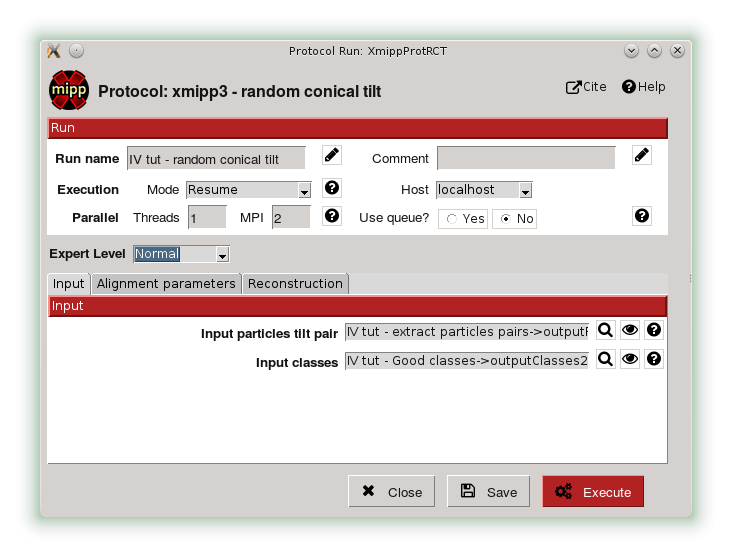
\includegraphics[width=0.75\textwidth]{{images/10.RCTprotocol}.png}
\caption{RCT protocol}
\label{RCTprotocol}
\end{figure}

\begin{figure}
\centering
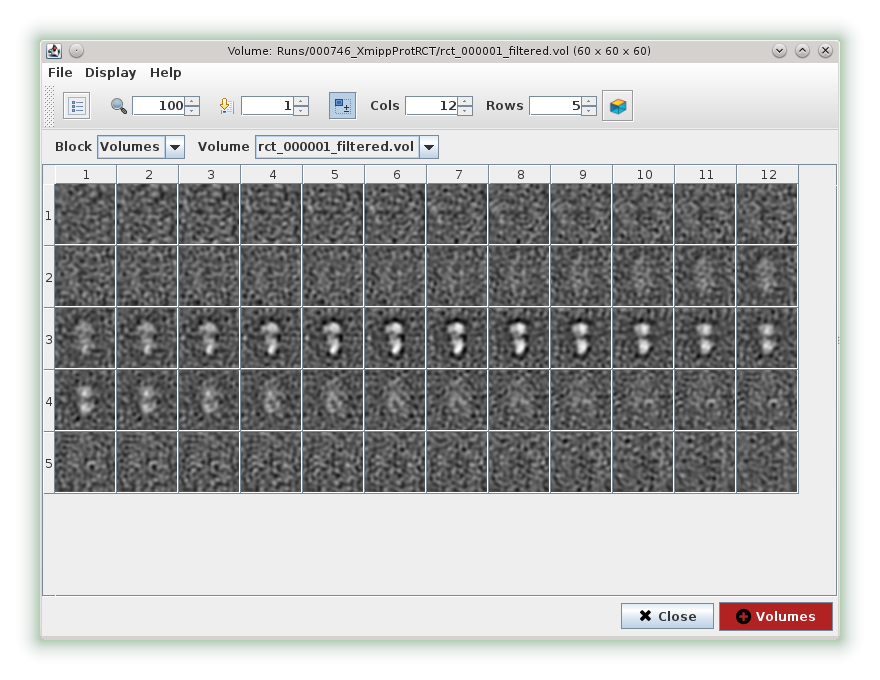
\includegraphics[width=0.75\textwidth]{{images/11.RCTresults}.png}
\caption{RCT output: Filtered volume.}
\label{RCTresults}
\end{figure}

This is enough to have our initial volume, but for having a better and more defined volume, we can also re-filter it 
by running the Xmipp Filter volumes protocol found under \textbf{3D - Preprocess} on the \textbf{Protocols SPA} view.
Protocol parameters are shown on figure ~\ref{VolFilter}

\begin{figure}
\centering
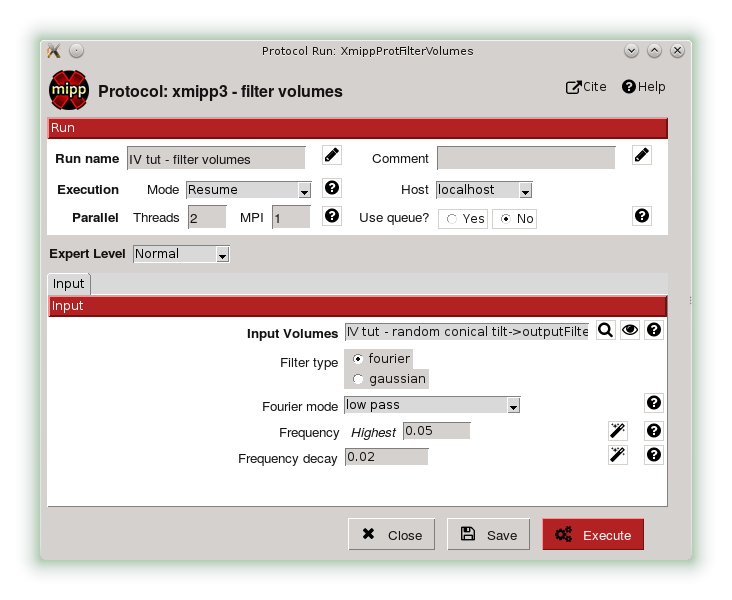
\includegraphics[width=0.75\textwidth]{{images/12.FilterVolsProtocol}.png}
\caption{Filter volume protocol.}
\label{VolFilter}
\end{figure}

\bibliographystyle{apalike}
\bibliography{../tutorial_initial_model/em.bib}

\end{document}